% =============================================================================
% Full paper: ML-Guided Route Selection for Carpooling Profit
% Copy this entire file into Overleaf. Upload figures to the same folder or set
% the path in \graphicspath{{./}} or {{figures/}}.
% =============================================================================

\documentclass[11pt,a4paper]{article}
\usepackage[utf8]{inputenc}
\usepackage[T1]{fontenc}
\usepackage{amsmath,amssymb}
\usepackage{graphicx}
\usepackage{booktabs}
\usepackage{hyperref}
\usepackage[margin=2.5cm]{geometry}
\usepackage{parskip}
\usepackage{tikz}
\usetikzlibrary{shapes.geometric,arrows.meta,positioning,fit,calc}
\usepackage{adjustbox}

% -----------------------------------------------------------------------------
% Title & author
% -----------------------------------------------------------------------------
\title{\textbf{Profit Prediction over Alternative Routes for Ride-Pooling:}\\[0.4em]
  \large Warm-Up vs.\ Cold-Start Route Selection with LightGBM and OSRM\\[0.3em]
  \normalsize Evidence from NYC TLC Taxi Data}
\author{Author Names Here\\
\texttt{email@example.com}}
\date{}

\begin{document}
\maketitle

\begin{abstract}
Real-time carpooling platforms must recommend a route within seconds. Default routing optimizes travel time and ignores rider demand and matching potential along alternative paths. We study whether machine learning--guided route selection (``warm-up'')---evaluating multiple road-network alternatives and choosing the route with highest predicted matching profit---yields higher platform profit than the naive strategy of accepting the default route (``cold-start'').

We use NYC TLC 2015 taxi data as a proxy for carpool demand: long trips as drivers, short trips as riders. For each driver we obtain three alternative routes from OSRM (Multi-Level Dijkstra), build H3-based corridors, and train a LightGBM model to predict post-matching profit per route using 38 non-leaky features (corridor geometry, temporal and spatial-demand signals, historical H3 statistics, landmark distances). Cold-start uses the default route; warm-up selects the route with highest predicted profit; we also evaluate random and heuristic baselines and an oracle (best actual profit) as an upper bound.

In a paired simulation on 5,000 test drivers with five random seeds, warm-up achieves higher mean profit than cold-start at every rider density level (100\%, 75\%, 50\%, 25\%, 10\%). The advantage increases as density decreases: +\$1.10 (3.7\%) at 100\% density and +\$2.21 (17.5\%) at 10\% density (paired $t$-test $p < 10^{-19}$; 95\% CIs reported). Rank-1 accuracy (predicted-best route = actual-best route) is 67.6\%. We conclude that route choice informed by predicted matching profit improves platform profit and that the effect is larger in sparser demand. All features use corridor candidates and historical H3 statistics only; no target leakage.

\noindent\textbf{Keywords:} ride-pooling, route choice, profit prediction, cold-start, spatial matching, H3, OSRM.
\end{abstract}

% =============================================================================
% 1. Introduction
% =============================================================================
\section{Introduction}

Carpooling platforms must recommend a route to the driver quickly. Standard routing engines return a default (e.g., fastest) path between origin and destination. That path ignores where riders are likely to be and how much revenue can be earned by matching riders along the way. A ``warm-up'' phase---requesting a small set of genuine road-network alternatives, predicting profit per route, and recommending the route with highest predicted profit---could increase platform revenue without increasing driver effort, but it has received limited empirical attention in the literature.

Prior work on ride-pooling often focuses on matching and assignment (e.g., Alonso-Mora et al.--style shareability \cite{alonso-mora}), optimization reviews \cite{agatz-review}, or route recommendation under different objective functions \cite{bassem-route}. Few studies isolate \textbf{route choice}---which of several alternative routes to recommend---for \textbf{profit} using \textbf{actual matching outcomes} and \textbf{real road networks}. We fill this gap with a simulation study on historical NYC TLC data. We compare two strategies: \textbf{cold-start} (use the default OSRM route) and \textbf{warm-up} (request three alternatives, predict profit per route with a LightGBM model, select the route with highest predicted profit; then match riders on the chosen route). To ensure a fair comparison, both strategies share the same OSRM request (three alternatives); cold-start's route is always one of warm-up's options.

\textbf{Contributions.}
\begin{enumerate}
\item \textbf{Paired experiment.} Same drivers, rider pool, and random seeds; only route-selection strategy differs. Cold-start uses the first route from a single OSRM \texttt{alternatives=3} response; warm-up ranks all three by predicted profit and selects the best. This design controls for driver and demand heterogeneity.
\item \textbf{Profit prediction with no leakage.} The model is trained on \textbf{post-matching} profit (matching is run during dataset construction). We use 38 features from route geometry, temporal context, corridor-level demand, historical H3 cell statistics, and landmark distances. We explicitly \textbf{exclude} matching-output features such as \texttt{matched\_rider\_count} and \texttt{feasible\_rider\_count}. An ablation study shows that temporal and corridor-demand features matter most.
\item \textbf{Density-dependent advantage.} We vary rider density (100\%, 75\%, 50\%, 25\%, 10\%) and show that the warm-up advantage \textbf{increases as density decreases}, with effect sizes and 95\% confidence intervals reported at each level (e.g., +\$1.10 at 100\%, +\$2.21 at 10\%).
\item \textbf{Multiple baselines and winner/loser analysis.} We report results for five strategies: cold-start, random (uniform over three routes), heuristic (highest corridor rider count), ML warm-up, and oracle (best actual profit). We report the fraction of drivers who are better off, tied, or worse off under warm-up, and the share of the oracle gap captured by ML.
\end{enumerate}

This study is a \textbf{simulation on historical data} (NYC TLC 2015), not a live deployment. The remainder of the paper is organized as follows: Section~\ref{sec:related} reviews related work; Section~\ref{sec:problem} formulates the problem and setting; Section~\ref{sec:method} describes the method; Section~\ref{sec:experiments} summarizes experiments and reproducibility; Section~\ref{sec:results} presents results; Section~\ref{sec:discussion} discusses limitations and threats to validity; Section~\ref{sec:conclusion} concludes.

% =============================================================================
% 2. Related Work
% =============================================================================
\section{Related Work}
\label{sec:related}

\textbf{Ride-pooling matching and optimization.} A large body of work studies matching and shareability in ride-pooling \cite{alonso-mora,agatz-atlanta,agatz-review,stiglic,chen-mcts}. Our setting differs: we \textbf{fix the route first} and then match riders on that route. We do not optimize over all possible route--rider assignments; we only choose which of three precomputed routes to recommend.

\textbf{Route choice and alternatives.} Multi-criteria routing and alternative-route generation (e.g., OSRM with MLD) are well established. Recent work has also studied carpool-oriented route recommendation \cite{bassem-route}. We use \textbf{road-network} alternatives and predict \textbf{profit} per route for selection, not only time or distance. Cold-start and warm-up share the same set of alternatives so that the comparison isolates the value of ML-based selection.

\textbf{Demand and profit prediction in mobility.} NYC TLC data have been used for demand, duration, and fare prediction (e.g., with XGBoost/LightGBM). We predict \textbf{driver--route profit} (revenue minus cost) at the \textbf{route} level, with the label defined as the \textbf{output of a matching engine} (no leakage from matching counts into features). In contrast to broader carpool optimization work that balances social or trust-based factors \cite{graal,srnc}, our objective is narrowly operational: route-level platform profit under a fixed matching rule.

\textbf{Spatial indexing (H3).} Uber H3 is used in ride-hailing for demand and dispatch. We use H3 for \textbf{corridor definition} (polyline $\to$ cells, k-ring expansion) and for a rider index keyed by (cell, 15-minute time bin). Pickup and dropoff must lie in the corridor; directionality and detour are enforced via geometric projection (Shapely).

% =============================================================================
% 3. Problem Formulation
% =============================================================================
\section{Problem Formulation and Setting}
\label{sec:problem}

\textbf{Actors.} A platform serves drivers (origin, destination, departure time) and riders (pickup, dropoff, time, fare). The platform must recommend \textbf{one} route from a small set (e.g., three) in seconds.

\textbf{Routes.} For each origin--destination pair we obtain the same set of alternatives (e.g., three OSRM routes). \textbf{Cold-start} uses the default (first) route. \textbf{Warm-up} uses a model to predict profit for each route and selects the route with highest predicted profit.

\textbf{Matching.} We define a corridor as the H3 (resolution 9) cells along the route polyline, expanded by one k-ring. Candidates are riders whose pickup and dropoff cells lie in the corridor and whose 15-minute time bin is within $\pm$1 bin of the driver's departure. Feasibility requires directionality (rider travels $\ge$5\% of route in driver direction), detour $\le$ 4 minutes, and seat capacity. Matching is greedy by fare with seed-based tie-breaking. \textbf{Profit} = platform\_share $\times$ sum(matched rider fares) $-$ route\_distance\_miles $\times$ cost\_per\_mile (platform\_share = 0.50, cost\_per\_mile = \$0.67).

\textbf{Objective.} We compare strategies by \textbf{expected profit per driver} (and related metrics), with proper aggregation and statistical tests.

\textbf{Data proxy.} We use NYC TLC Yellow Taxi 2015 trips as a proxy for carpool demand: long trips ($>$10 mi) as drivers, short trips (0.5--10 mi) as riders. This choice and its limitations are revisited in the Discussion.

% =============================================================================
% 4. Method
% =============================================================================
\section{Method}
\label{sec:method}

\subsection{System Architecture}
\label{sec:architecture}

Figure~\ref{fig:architecture} summarizes the end-to-end pipeline. The OSRM MLD server (Docker, localhost) holds the New York road network and returns 2--3 genuine alternative routes per origin--destination request. All responses are cached in SQLite (\texttt{route\_cache.db}), so the simulation runs in cache-only mode with no live API calls. For each driver, the cache supplies up to three route polylines. Three shared components then operate on these routes:

\begin{itemize}
\item \textbf{Corridor builder:} For each polyline, we densify at 80\,m steps, map points to H3 resolution-9 cells, and expand by one k-ring to form a corridor ($\sim$520\,m width). Output: the set of H3 cells that define the spatial catchment for that route.
\item \textbf{Matcher (Shapely/GEOS):} Given a corridor and a route polyline, the matcher (Section~\ref{sec:matching}) finds riders whose pickup and dropoff lie in the corridor and satisfy directionality, detour, and seat constraints; it then assigns seats greedily by fare. This is used both for generating training labels (profit per route) and for simulating cold-start and warm-up outcomes.
\item \textbf{LightGBM predictor:} For each of the three routes we compute 38 features (geometry, temporal, corridor demand, historical H3, landmarks, cell-level). The model predicts profit per route; warm-up selects the route with highest predicted profit.
\end{itemize}

Cold-start uses only the first route (default) and runs the matcher once. Warm-up runs the corridor builder and feature extraction for all three routes, invokes the predictor to rank them, then runs the matcher once on the selected route. The runner executes both strategies for each driver over 5 seeds (driver-major loop), then aggregates outcomes and runs statistical tests and visualizations. This architecture ensures that cold-start's route is always one of warm-up's options, so the comparison is fair.

% --- Figure 1: System Architecture (TikZ) ---
\begin{figure}[htbp]
\centering
\resizebox{\textwidth}{!}{%
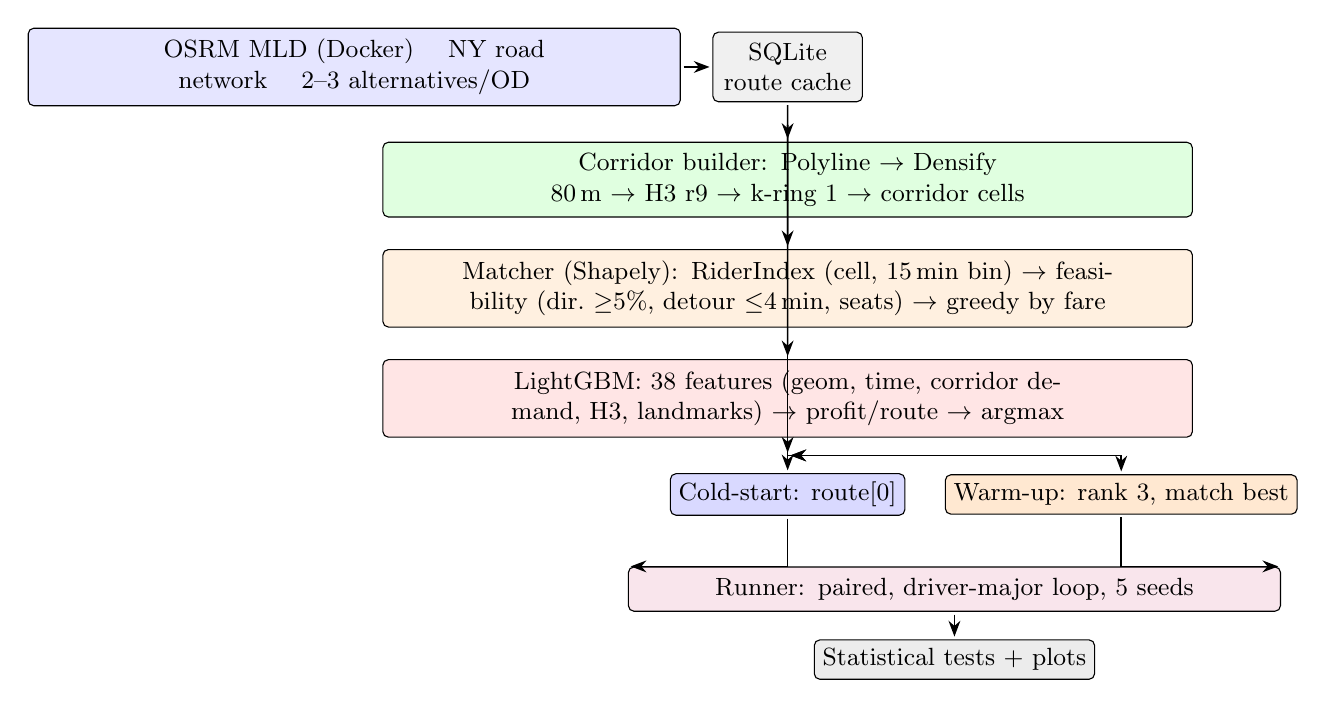
\begin{tikzpicture}[
  node distance=0.45cm and 0.35cm,
  font=\small,
  box/.style={rectangle, draw, rounded corners=2pt, inner sep=4pt, align=center},
  comp/.style={box, text width=10cm, minimum height=0.75cm},
  smallbox/.style={box, minimum height=0.5cm, inner sep=3pt},
  arrow/.style={-Stealth, semithick, shorten >=1pt, shorten <=1pt}
]
  % Row 1: OSRM -> Cache
  \node[box, fill=blue!10, minimum height=0.65cm, text width=8cm] (osrm) {OSRM MLD (Docker) \quad NY road network \quad 2--3 alternatives/OD};
  \node[box, right=0.4cm of osrm, fill=gray!12, minimum width=1.3cm, minimum height=0.65cm] (cache) {SQLite\\route cache};
  \draw[arrow] (osrm.east) -- (cache.west);

  % Row 2: three components stacked vertically (text width forces wrap, stays in column)
  \node[comp, below=0.5cm of cache, fill=green!12, anchor=north] (corr) {Corridor builder: Polyline $\to$ Densify 80\,m $\to$ H3 r9 $\to$ k-ring 1 $\to$ corridor cells};
  \node[comp, below=0.4cm of corr, fill=orange!12, anchor=north] (match) {Matcher (Shapely): RiderIndex (cell, 15\,min bin) $\to$ feasibility (dir.\ $\ge$5\%, detour $\le$4\,min, seats) $\to$ greedy by fare};
  \node[comp, below=0.4cm of match, fill=red!10, anchor=north] (lgb) {LightGBM: 38 features (geom, time, corridor demand, H3, landmarks) $\to$ profit/route $\to$ argmax};

  % Cache -> three components: one vertical trunk then branch to each
  \coordinate (cachebot) at ($(cache.south)!0.5!(corr.north)$);
  \draw[arrow] (cache.south) -- (cachebot) -- (corr.north);
  \draw[arrow] (cachebot) -- (match.north);
  \draw[arrow] (cachebot) -- (lgb.north);

  % Row 3: strategies; single junction below lgb, then branch to cs and wu
  \node[smallbox, below=0.45cm of lgb, fill=blue!15, minimum width=2cm, anchor=north] (cs) {Cold-start: route[0]};
  \node[smallbox, right=0.5cm of cs, fill=orange!18, minimum width=2.2cm] (wu) {Warm-up: rank 3, match best};
  \coordinate (junc) at ($(lgb.south)!0.5!(cs.north)$);
  \draw[arrow] (corr.south) -- (corr.south |- junc) -- (junc);
  \draw[arrow] (match.south) -- (match.south |- junc) -- (junc);
  \draw[arrow] (lgb.south) -- (junc);
  \draw[arrow] (junc) -| (cs.north);
  \draw[arrow] (junc) -| (wu.north);

  % Row 4: runner (centered under cs and wu); right-angled arrows (down then horizontal)
  \node[comp, below=0.45cm of $(cs.south)!0.5!(wu.south)$, fill=purple!10, text width=8cm, minimum height=0.55cm, anchor=north, yshift=-0.2cm] (runner) {Runner: paired, driver-major loop, 5 seeds};
  \draw[arrow] (cs.south) -- (cs.south |- runner.north) -- (runner.north west);
  \draw[arrow] (wu.south) -- (wu.south |- runner.north) -- (runner.north east);

  % Row 5: output
  \node[smallbox, below=0.35cm of runner, fill=gray!15, minimum width=2.5cm] (stats) {Statistical tests + plots};
  \draw[arrow] (runner.south) -- (stats.north);
\end{tikzpicture}%
}
\caption{System architecture. OSRM MLD supplies 2--3 alternative routes per OD; the SQLite cache serves them to the corridor builder (polyline $\to$ densify 80\,m $\to$ H3 r9 $\to$ k-ring 1), matcher (RiderIndex $\to$ Shapely feasibility $\to$ greedy by fare), and LightGBM predictor (38 features $\to$ profit per route $\to$ argmax). Cold-start uses the default route; warm-up ranks all three and matches on the selected route. The runner executes both strategies per driver over 5 seeds, then aggregates and runs tests.}
\label{fig:architecture}
\end{figure}

\subsection{Data and Preprocessing}

We use NYC TLC Yellow Taxi 2015 (Azure Open Datasets). \textbf{Temporal split:} January--March for training, April for test; no test period appears in training. \textbf{Drivers:} trips with trip\_distance\_miles $>$ 10. \textbf{Riders:} trips 0.5--10 mi, 25\% sample. We assign H3 (resolution 9) cells to pickup and dropoff and use 15-minute bins for the rider index. All preprocessing is documented in the project README.

\subsection{Spatial and Routing}

We use OSRM with the Multi-Level Dijkstra (MLD) algorithm on a New York road graph (Docker). MLD returns 2--3 genuine alternative routes per request. Routes are cached in SQLite so experiments are reproducible without live routing calls.

\textbf{Corridor construction (Figure~\ref{fig:corridor-pipeline}).} A corridor is the spatial band around a route where rider pickups and dropoffs are considered matchable. The pipeline is: (1) \textbf{Polyline} --- OSRM returns a sequence of (lat, lng) points along the road. (2) \textbf{Densify} --- We interpolate points every 80\,m along the polyline. At H3 resolution 9 (hex edge $\sim$174\,m), 80\,m steps guarantee no cell is skipped between consecutive points. (3) \textbf{H3 cells} --- Each interpolated point is mapped to its H3 resolution-9 cell; we keep the ordered list of cells along the route (the ``spine''). (4) \textbf{k-ring expand (k=1)} --- For each spine cell we add all 6 adjacent cells via H3's grid disk. The union of spine and neighbors forms the corridor: a band of width $\sim$520\,m around the road.

Resolution 9 and k=1 yield a catchment consistent with a short walk to the road ($\sim$500\,m). Figure~\ref{fig:corridor-map} illustrates this for one long origin--destination pair: three alternative routes and their H3 corridors are overlaid on a map; the differing coverage of the road network explains why route choice affects which riders can be matched.

% --- Figure 2: Corridor construction (TikZ) ---
\begin{figure}[htbp]
\centering
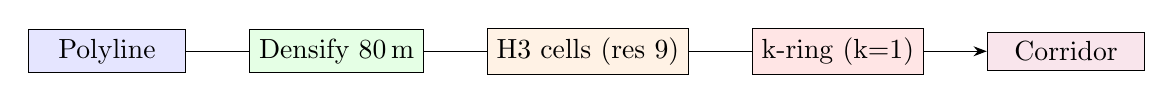
\begin{tikzpicture}[node distance=0.8cm, box/.style={rectangle, draw, minimum width=2cm}, arrow/.style={-Stealth}]
  \node[box, fill=blue!10] (p) {Polyline};
  \node[box, right=of p, fill=green!10] (d) {Densify 80\,m};
  \node[box, right=of d, fill=orange!10] (h) {H3 cells (res 9)};
  \node[box, right=of h, fill=red!10] (k) {k-ring (k=1)};
  \node[box, right=of k, fill=purple!10] (c) {Corridor};
  \draw[arrow] (p) -- (d) -- (h) -- (k) -- (c);
\end{tikzpicture}
\caption{Corridor construction pipeline. The route polyline is densified every 80\,m, each point is mapped to an H3 resolution-9 cell, and a one-step k-ring expansion produces a band of width $\sim$520\,m around the route.}
\label{fig:corridor-pipeline}
\end{figure}

\subsection{Matching Pipeline}
\label{sec:matching}

Figure~\ref{fig:matching-pipeline} outlines the three-stage flow from corridor and route to matched riders and profit. The same pipeline is used for generating training labels and for simulating cold-start and warm-up.

\textbf{Stage 1 --- Spatial--temporal filter (RiderIndex).} We maintain an in-memory index mapping (H3 cell, 15-minute time bin) to rider indices. For a given corridor (set of H3 cells) and driver departure time, we query riders whose pickup cell and dropoff cell both lie in the corridor and whose 15-min bin is within $\pm$1 bin of the driver's bin (45-minute window). This reduces the full rider set (millions) to on the order of 10--50 candidates per route.

\textbf{Stage 2 --- Feasibility filter (Shapely/GEOS).} For each candidate we (a) project pickup and dropoff onto the route polyline using line\_locate\_point (normalized 0--1); (b) require dropoff\_frac $-$ pickup\_frac $\ge$ 0.05 (rider travels at least 5\% of the route in the driver's direction); (c) compute perpendicular distances to the route and estimate detour as $2 \times (\text{pickup\_perp} + \text{dropoff\_perp}) \times 1.3 / (40\,\text{km/h})$, and require detour $\le$ 4 minutes; (d) require passenger\_count $\le$ remaining seats (3). Coordinates are scaled by $\cos(\text{lat})$ for NYC so that Shapely distances approximate meters. Output: typically 2--5 feasible riders.

\textbf{Stage 3 --- Greedy assignment.} Feasible riders are sorted by fare descending, with a small random perturbation ($\pm$\$0.01) per rider for seed-based tie-breaking. We assign seats greedily until capacity (3) is reached. The result is 0--3 matched riders. \textbf{Profit} = platform\_share $\times$ sum(matched rider fares) $-$ route\_distance\_miles $\times$ cost\_per\_mile (platform\_share = 0.50, cost\_per\_mile = \$0.67).

\textbf{Label for training:} For each (driver, route) we run this full pipeline and set the \textbf{label} to the resulting profit. We do \textbf{not} use the sum of all corridor rider fares; that would ignore capacity, directionality, and detour and would produce a 1000$\times$ inflated label.

% --- Figure 3: Matching pipeline (TikZ) ---
\begin{figure}[htbp]
\centering
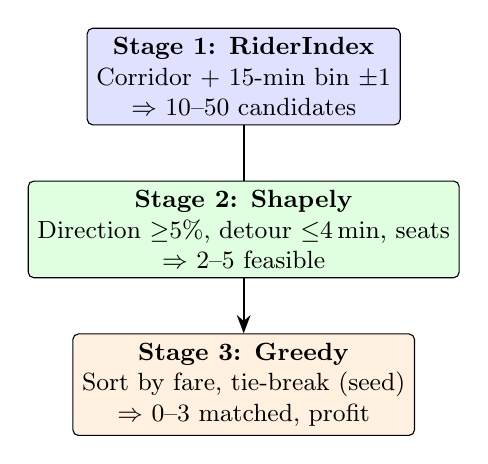
\begin{tikzpicture}[
  node distance=0.7cm,
  stage/.style={rectangle, draw, rounded corners=2pt, minimum width=3.2cm, minimum height=0.9cm, font=\small, align=center},
  arrow/.style={-Stealth, thick}
]
  \node[stage, fill=blue!12] (s1) {\textbf{Stage 1: RiderIndex}\\Corridor + 15-min bin $\pm$1\\$\Rightarrow$ 10--50 candidates};
  \node[stage, below=of s1, fill=green!12] (s2) {\textbf{Stage 2: Shapely}\\Direction $\ge$5\%, detour $\le$4\,min, seats\\$\Rightarrow$ 2--5 feasible};
  \node[stage, below=of s2, fill=orange!12] (s3) {\textbf{Stage 3: Greedy}\\Sort by fare, tie-break (seed)\\$\Rightarrow$ 0--3 matched, profit};
  \draw[arrow] (s1) -- (s2) -- (s3);
\end{tikzpicture}
\caption{Matching pipeline. Stage 1: spatial--temporal filter via RiderIndex. Stage 2: feasibility filter (directionality, detour, seat capacity) using Shapely. Stage 3: greedy assignment by fare with seed-based tie-breaking; output is matched riders and profit.}
\label{fig:matching-pipeline}
\end{figure}

\subsection{Profit Prediction Model}

\textbf{Label:} Per (driver, route), run matching $\to$ profit. \textbf{Features (38):} Geometric (distance, duration, corridor cells, sinuosity, speed, bearing, straight-line distance), temporal (hour, day of week, weekend, day of month, 15-min bin, hour sin/cos), corridor demand (rider count in corridor, demand density, mean fare, fare density), historical H3 (pickups, dropoffs, densities, mean fare, fare density per corridor), landmark distances (JFK, LGA, Penn, Times Square; nearest landmark), and cell-level (origin/dest cell pickups/dropoffs and mean fare). We \textbf{exclude} \texttt{matched\_rider\_count} and \texttt{feasible\_rider\_count}. \textbf{Model:} LightGBM regressor. \textbf{Validation:} GroupShuffleSplit by driver\_id (80/20) so no driver appears in both train and validation. \textbf{Inference:} Predict profit for each of three routes; recommend argmax. \textbf{Metrics:} $R^2$ and RMSE on validation; \textbf{rank-1 accuracy} = fraction of drivers for whom the route with highest predicted profit equals the route with highest actual profit.

\subsection{Strategies}

\textbf{Cold-start:} Use routes[0]. \textbf{Random:} Uniform over the three routes. \textbf{Heuristic:} Route with highest corridor\_rider\_count. \textbf{ML warm-up:} Route with highest predicted profit. \textbf{Oracle:} Run matching on all three routes; pick the route with highest actual profit (upper bound). All strategies use the same OSRM \texttt{alternatives=3} response; cold-start's route is always in warm-up's set.

\subsection{Experimental Design}

\textbf{Paired:} Same drivers, same rider pool, same seeds; only strategy varies. We use 5 seeds; outcomes are aggregated to \textbf{per-driver means} over seeds before running statistical tests (no pseudoreplication). \textbf{Density experiments:} Same test drivers; rider set is subsampled to 100\%, 75\%, 50\%, 25\%, and 10\% (fixed seed). Each density level yields a full set of strategy outcomes.

% =============================================================================
% 5. Experiments
% =============================================================================
\section{Experiments and Reproducibility}
\label{sec:experiments}

\textbf{Scale.} Training dataset: $\sim$218K rows (from $\sim$100K drivers, $\sim$2.18 routes per driver). Test: 5,000 drivers $\times$ 5 seeds $\times$ 5 strategies. Density runs: same 5,000 drivers at each of five density levels.

\textbf{Software.} Python 3.10+, OSRM (Docker), H3, Shapely (GEOS), LightGBM, scikit-learn, scipy. Route cache: SQLite. Exact commands for dataset build, training, simulation, and plotting are documented in the repository (README and PAPER\_PLAN).

\textbf{Reproducibility.} Sequence: (1) preprocess data $\to$ (2) build training dataset (with matching for labels) $\to$ (3) train model $\to$ (4) run simulation (cache-only) $\to$ (5) generate figures and summaries. Commit/tag and environment (e.g., requirements.txt) allow replication. Runtime: dataset build on the order of hours; training minutes; simulation on the order of hours for 5K drivers $\times$ 5 seeds $\times$ 5 strategies.

% =============================================================================
% 6. Results
% =============================================================================
\section{Results}
\label{sec:results}

\subsection{Main Result: Warm-Up vs Cold-Start by Density}

Table~\ref{tab:density} reports mean profit (cold-start and warm-up), mean difference (warm-up $-$ cold-start), 95\% CI for the mean difference (t-based: mean $\pm$ 1.96$\times$SEM of driver-level differences), and percentage gain at each rider density. Sample size: 5,000 drivers; per-driver values are means over 5 seeds.

\begin{table}[htbp]
\centering
\caption{Mean profit and warm-up advantage by rider density (5,000 drivers, 5 seeds). 95\% CI = mean difference $\pm$ 1.96$\times$SEM (driver-level differences).}
\label{tab:density}
\begin{tabular}{lrrrrr}
\toprule
Density & Cold-Start (\$) & Warm-Up (\$) & Mean $\Delta$ (\$) & 95\% CI ($\Delta$) & \% Gain \\
\midrule
100\% & 29.90 & 31.01 & 1.10 & [0.87, 1.34] & 3.7\% \\
75\%  & 27.94 & 29.14 & 1.20 & [0.96, 1.43] & 4.3\% \\
50\%  & 24.88 & 26.15 & 1.27 & [1.05, 1.49] & 5.1\% \\
25\%  & 19.60 & 21.23 & 1.64 & [1.42, 1.86] & 8.4\% \\
10\%  & 12.67 & 14.88 & 2.21 & [2.00, 2.42] & 17.5\% \\
\bottomrule
\end{tabular}
\end{table}

At 100\% density, paired $t$-test $t = 9.24$, $p = 3.51 \times 10^{-20}$; Wilcoxon $W = 651696$, $p = 5.55 \times 10^{-23}$. The warm-up advantage increases monotonically as rider density decreases; at 10\% density the gain is +\$2.21 (17.5\%).

\subsection{Strategy Comparison (100\% Density)}

Table~\ref{tab:strategies} reports mean profit (and vs cold-start) for all five strategies at 100\% rider density.

\begin{table}[htbp]
\centering
\caption{Strategy comparison at 100\% rider density (5,000 drivers).}
\label{tab:strategies}
\begin{tabular}{lrrl}
\toprule
Strategy & Mean profit (\$) & \multicolumn{1}{c}{vs Cold-Start} \\
\midrule
Cold-Start & 29.90 & --- \\
Random     & 29.05 & $-\$0.85$ \\
Heuristic  & 30.91 & $+\$1.00$ \\
ML Warm-Up & 31.01 & $+\$1.10$ \\
Oracle     & 33.87 & $+\$3.97$ \\
\bottomrule
\end{tabular}
\end{table}

Oracle advantage over cold-start is \$3.97; ML captures \$1.10, i.e., \textbf{27.8\%} of the oracle gap. Random performs worse than cold-start; heuristic captures most of the gain; ML warm-up slightly outperforms heuristic by only \textbf{\$0.10/trip} at 100\% density.

\subsection{Who Benefits}

From extended summary (100\% density): \textbf{23.3\%} of drivers are better off with warm-up, \textbf{62.4\%} tied, \textbf{14.3\%} worse off. Mean gain among winners: \$10.20; mean loss among losers: \$8.96. Effect size (Cohen's $d$) = 0.069 (negligible by conventional rules); 95\% CI for mean difference (bootstrap): [\$0.87, \$1.34].

\subsection{Density and Advantage}

Figure~\ref{fig:density} plots rider density (x) vs mean profit difference warm-up $-$ cold-start (y) with 95\% CI. The curve is increasing as density decreases, supporting the message that \textbf{route choice matters more when rider availability is sparser}.

\begin{figure}[htbp]
\centering
\includegraphics[width=0.85\textwidth]{paper_fig1_density_advantage.png}
\caption{Warm-up advantage over cold-start by rider density. Mean profit difference (WU$-$CS) with 95\% CI. Sample: 5,000 drivers, 5 seeds.}
\label{fig:density}
\end{figure}

\subsection{Model Quality}

Validation $R^2 \approx 0.79$, RMSE $\approx$ \$7.92; rank-1 accuracy is approximately 68\%. Top features by importance: corridor\_fare\_density, time\_bin\_15min, mean\_rider\_fare. Figure~\ref{fig:model} shows feature importance and predicted vs actual profit on the validation set.

\begin{figure}[htbp]
\centering
\includegraphics[width=\textwidth]{paper_fig4_model_quality.png}
\caption{Profit model: top 15 feature importance and predicted vs actual (validation). $R^2 \approx 0.79$, RMSE $\approx$ \$7.92, rank-1 accuracy $\approx 68\%$.}
\label{fig:model}
\end{figure}

Table~\ref{tab:ablation} gives model validation and feature ablation (GroupShuffleSplit by driver\_id). Removing temporal features causes the largest drop; spatial-demand and geometric groups also contribute substantially.

\begin{table}[htbp]
\centering
\caption{Model validation and feature ablation (GroupShuffleSplit by driver\_id).}
\label{tab:ablation}
\small
\begin{tabular}{llrrr}
\toprule
Experiment & Features & $R^2$ & RMSE & Rank-1 \\
\midrule
All features        & 38 & 0.7925 & \$7.92  & 67.9\% \\
Only Geometric      & 8  & 0.3292 & \$14.23 & 54.6\% \\
Only Temporal       & 7  & 0.1042 & \$16.45 & 46.5\% \\
Only Spatial Demand & 13 & 0.5547 & \$11.60 & 60.8\% \\
Only Landmark       & 10 & 0.3247 & \$14.28 & 46.5\% \\
All minus Geometric & 30 & 0.7893 & \$7.98  & 66.9\% \\
All minus Temporal  & 31 & 0.5522 & \$11.63 & 60.9\% \\
All minus Spatial   & 25 & 0.7346 & \$8.95  & 61.9\% \\
All minus Landmark  & 28 & 0.7839 & \$8.08  & 67.6\% \\
\bottomrule
\end{tabular}
\end{table}

% --- Additional figures: strategy comparison, profit difference, profit by density, corridor map ---
\begin{figure}[htbp]
\centering
\includegraphics[width=0.85\textwidth]{paper_fig2_strategy_comparison.png}
\caption{Strategy comparison: mean profit with 95\% CI at 100\% rider density (5,000 drivers).}
\label{fig:strategy}
\end{figure}

\begin{figure}[htbp]
\centering
\includegraphics[width=0.85\textwidth]{paper_fig3_profit_difference.png}
\caption{Distribution of per-driver profit difference (Warm-Up $-$ Cold-Start), overall and by route length.}
\label{fig:profit-diff}
\end{figure}

\begin{figure}[htbp]
\centering
\includegraphics[width=0.85\textwidth]{paper_fig5_profit_by_density.png}
\caption{Mean profit by strategy (Cold-Start, ML Warm-Up, Oracle) across rider density levels.}
\label{fig:profit-by-density}
\end{figure}

\begin{figure}[htbp]
\centering
\includegraphics[width=0.9\textwidth]{paper_fig6_corridor_map.png}
\caption{Three alternative routes and their H3 corridors for one long origin--destination pair. Illustrates how corridor coverage differs by route and why route choice affects matchability.}
\label{fig:corridor-map}
\end{figure}

% =============================================================================
% 7. Discussion
% =============================================================================
\section{Discussion}
\label{sec:discussion}

\textbf{Interpretation.} Warm-up improves mean profit by selecting routes with higher predicted matching profit. Temporal and corridor-demand features drive the model. The advantage grows when rider availability is sparser (lower density), where route choice has a larger impact on who can be matched. At the same time, the small gap between the heuristic and ML baselines at 100\% density suggests that the main signal is route-aware demand ranking, while the incremental value of the full ML model over a simple count-based heuristic is modest in this saturated NYC setting.

\textbf{Limitations.} (1) Static snapshot; no dynamic arrivals or cancellations. (2) Taxi data as proxy for carpool demand. (3) Single city and period (NYC, April 2015). (4) Driver always accepts the recommended route. (5) Fixed platform share and cost. (6) Temporal train/test (conservative). (7) At 100\% density, match rates are high for both strategies ($\sim$99\%), limiting the visible advantage; at 10\% density the gain is much larger.

\textbf{Threats to validity.} Internal: paired design and shared OSRM set reduce confounds. External: generalization to other cities or time periods is unknown. Construct: profit is platform profit; other objectives (e.g., driver or rider welfare) could be studied separately.

\textbf{Future work.} Pairwise or relative features between routes; multi-city evaluation; dynamic setting; live A/B test; other objectives (e.g., emissions, fairness).

% =============================================================================
% 8. Conclusion
% =============================================================================
\section{Conclusion}
\label{sec:conclusion}

We showed that ML-guided route selection (warm-up) yields higher mean profit than default routing (cold-start) in a simulation on NYC TLC 2015 data. The effect is statistically significant (paired $t$ and Wilcoxon $p < 10^{-19}$), with a mean difference of +\$1.10 at 100\% rider density and +\$2.21 at 10\% density. Rank-1 accuracy is 67.6\%; ML captures about 28\% of the oracle gap. The advantage increases as rider density decreases, indicating that route choice is a lever for platform profit especially in sparser demand. The study is limited to a single city and historical simulation; implications for deployment would require real-world validation.

% =============================================================================
% Acknowledgments (optional)
% =============================================================================
\begin{thebibliography}{99}
\bibitem{alonso-mora}
J. Alonso-Mora, S. Samaranayake, A. Wallar, E. Frazzoli, and D. Rus, ``On-demand high-capacity ride-sharing via dynamic trip-vehicle assignment,'' \textit{Proceedings of the National Academy of Sciences}, vol.~114, no.~3, pp.~462--467, 2017.

\bibitem{agatz-review}
N. Agatz, A. Erera, M. Savelsbergh, and X. Wang, ``Optimization for dynamic ride-sharing: A review,'' \textit{European Journal of Operational Research}, vol.~223, no.~2, pp.~295--303, 2012.

\bibitem{agatz-atlanta}
N. Agatz, A. Erera, M. Savelsbergh, and X. Wang, ``Dynamic ride-sharing: A simulation study in metro Atlanta,'' \textit{Transportation Research Part B: Methodological}, vol.~45, no.~9, pp.~1450--1464, 2011.

\bibitem{stiglic}
M. Stiglic, N. Agatz, M. Savelsbergh, and M. Gradisar, ``Making dynamic ride-sharing work: The impact of driver and rider flexibility,'' \textit{Transportation Research Part E: Logistics and Transportation Review}, vol.~91, pp.~190--207, 2016.

\bibitem{bassem-route}
C. Bassem, S. Honcharuk, and M. F. Mokbel, ``Route Recommendation to Facilitate Carpooling,'' in \textit{Proceedings of the 23rd IEEE International Conference on Mobile Data Management (MDM)}, pp.~29--34, 2022.

\bibitem{graal}
M. Berlingerio, B. Ghaddar, R. Guidotti, A. Pascale, and A. Sassi, ``The GRAAL of carpooling: GReen And sociAL optimization from crowd-sourced data,'' \textit{Transportation Research Part C: Emerging Technologies}, vol.~80, pp.~20--36, 2017.

\bibitem{srnc}
J. Xia, K. M. Curtin, J. Huang, D. Wu, W. Xiu, and Z. Huang, ``A carpool matching model with both social and route networks,'' \textit{Computers, Environment and Urban Systems}, vol.~75, pp.~90--102, 2019.

\bibitem{chen-mcts}
X. Chen, H. Zheng, F. Xiao, and X. Chen, ``Efficient dispatching for on-demand ride services: Systematic optimization via Monte-Carlo tree search,'' \textit{Transportation Research Part C: Emerging Technologies}, vol.~127, art.~103156, 2021.

\bibitem{osrm}
OSRM, ``Project OSRM,'' \url{https://project-osrm.org}.

\bibitem{h3}
Uber Engineering, ``H3: Uber's Hexagonal Hierarchical Spatial Index,'' \url{https://eng.uber.com/h3}.

\bibitem{lightgbm}
G. Ke et al., ``LightGBM: A highly efficient gradient boosting decision tree,'' in \textit{Advances in Neural Information Processing Systems}, vol.~30, 2017.

\bibitem{nyctlc}
NYC TLC, ``Trip Record Data,'' Azure Open Datasets, \url{https://learn.microsoft.com/en-us/azure/open-datasets/dataset-taxi-green?tabs=azure-storage}.
\end{thebibliography}

\end{document}
